\chapter{Implementing the SoC}
\minitoc
\newpage

\setcounter{secnumdepth}{0} % Set the section counter to 0 so next section is not counted in toc
% ----------------------- Introduction ----------------------- %
\section{Introduction}
In this chapter, we will discuss the implementation of the Security Operation Center (SoC) that we designed in the previous chapter.
We will use Security Onion for the main center of operations and GNS3 to emulate the network environment.

\setcounter{secnumdepth}{2} % Resume counting the sections for the toc with a depth of 2 (Sections and sub-sections)
% ----------------------------------- SECTIONS (v) ----------------------------------- %
% ----------------------- Network Environment Setup ----------------------- %
\section{Network Environment Setup}
To start it off, we created a network topology in GNS3 that includes a pfSense firewall, acting as the gateway to the network, and multiple endpoints and servers as shown in the figure below.
The internet is simulated using a cloud node in GNS3 and it will just connect to the local network though a virtual bridge.

\begin{figure}[H]
    \centering
    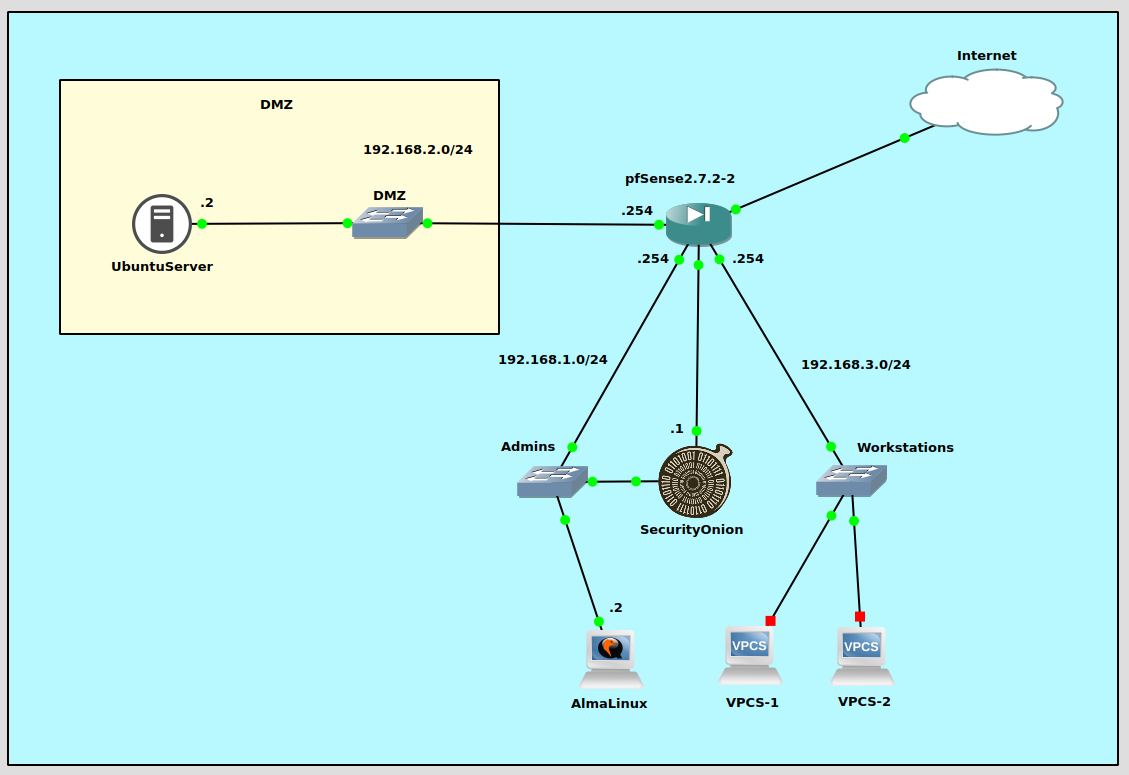
\includegraphics[width=1\textwidth]{src/assets/diagrams/gns3-topology.png}
    \caption{Network Topology in GNS3}
\end{figure}

% ----------------------- Security Onion ----------------------- %
\section{Security Onion}

\subsection{Definition}
Security Onion is a free and open-source Linux distribution for threat hunting, enterprise security monitoring, and log management.
It includes Elasticsearch, Logstash, Kibana, Snort, Suricata, Zeek, Wazuh, TheHive, CyberChef, and many other security tools.

This is the brain of our SoC, where all the data from the network will be collected, analyzed, and responded to.

\subsection{Installation}
Following the official documentation of Security Onion, we installed the latest version of the software in a QEMU virtual machine directly inside GNS3.
The installation process was quite straightforward after solving a very specific problem that will be mentioned later, but it required a lot of disk space and resources.

\begin{figure}[H]
    \centering
    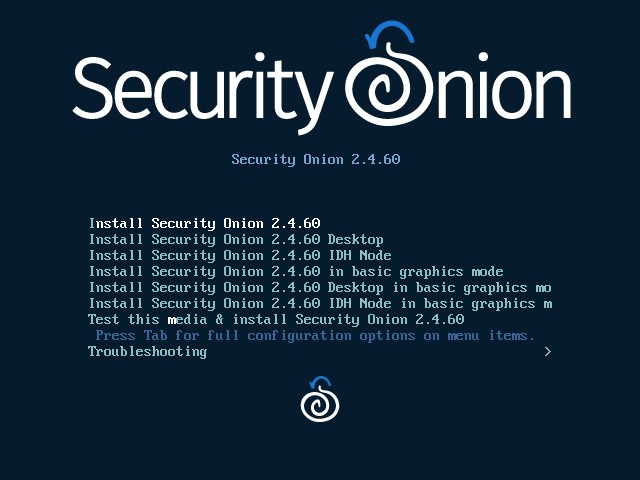
\includegraphics[width=10cm]{src/assets/images/security-onion-install.jpg}
    \caption{Installation wizard of Security Onion}
\end{figure}

\begin{table}[H]
    \renewcommand{\arraystretch}{1.5}%
    \caption{Minimum Requirements of Security Onion 2}
    \centering
    \medskip
    \begin{tabularx}{1\textwidth} {
            | >{\hsize=1\hsize\linewidth=\hsize\centering\arraybackslash}X
            | >{\hsize=1\hsize\linewidth=\hsize\centering\arraybackslash}X
            | >{\hsize=1\hsize\linewidth=\hsize\centering\arraybackslash}X
            | >{\hsize=1\hsize\linewidth=\hsize\centering\arraybackslash}X
            | >{\hsize=1\hsize\linewidth=\hsize\centering\arraybackslash}X |}
        \hline
        \rowcolor{primary} \textbf{Type} & \textbf{CPUs} & \textbf{RAM} & \textbf{Storage} & \textbf{NICs} \\
        \hline
        Eval                             & 4             & 12GB         & 200GB            & 2             \\
        \hline
        Standalone                       & 4             & 16GB         & 200GB            & 2             \\
        \hline
    \end{tabularx}
\end{table}

There is a subtle difference between the "Eval" and "Standalone" installations, the former is for evaluation purposes and the latter is for production environments.
There are more types available bu we only mentioned the two that are relevant to our project.

We picked the "Standalone" installation.

\begin{figure}[H]
    \centering
    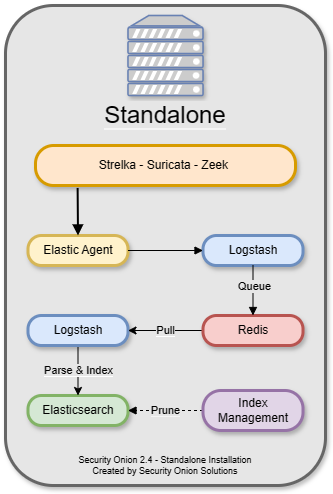
\includegraphics[width=7cm]{src/assets/diagrams/security-onion-standalone.png}
    \caption{Security Onion Standalone Architecture}
\end{figure}

"Standalone is similar to Evaluation in that all components run on one box.
However, instead of Elastic Agent sending logs directly to Elasticsearch, it sends them to Logstash, which sends them to Redis for queuing.
A second Logstash pipeline pulls the logs out of Redis and sends them to Elasticsearch, where they are parsed and indexed." - \cite{security-onion-docs}

\subsection{Interface}
After the installation, we accessed the Security Onion interface through a web browser and configured the network interfaces to monitor the traffic on the network.

\begin{figure}[H]
    \centering
    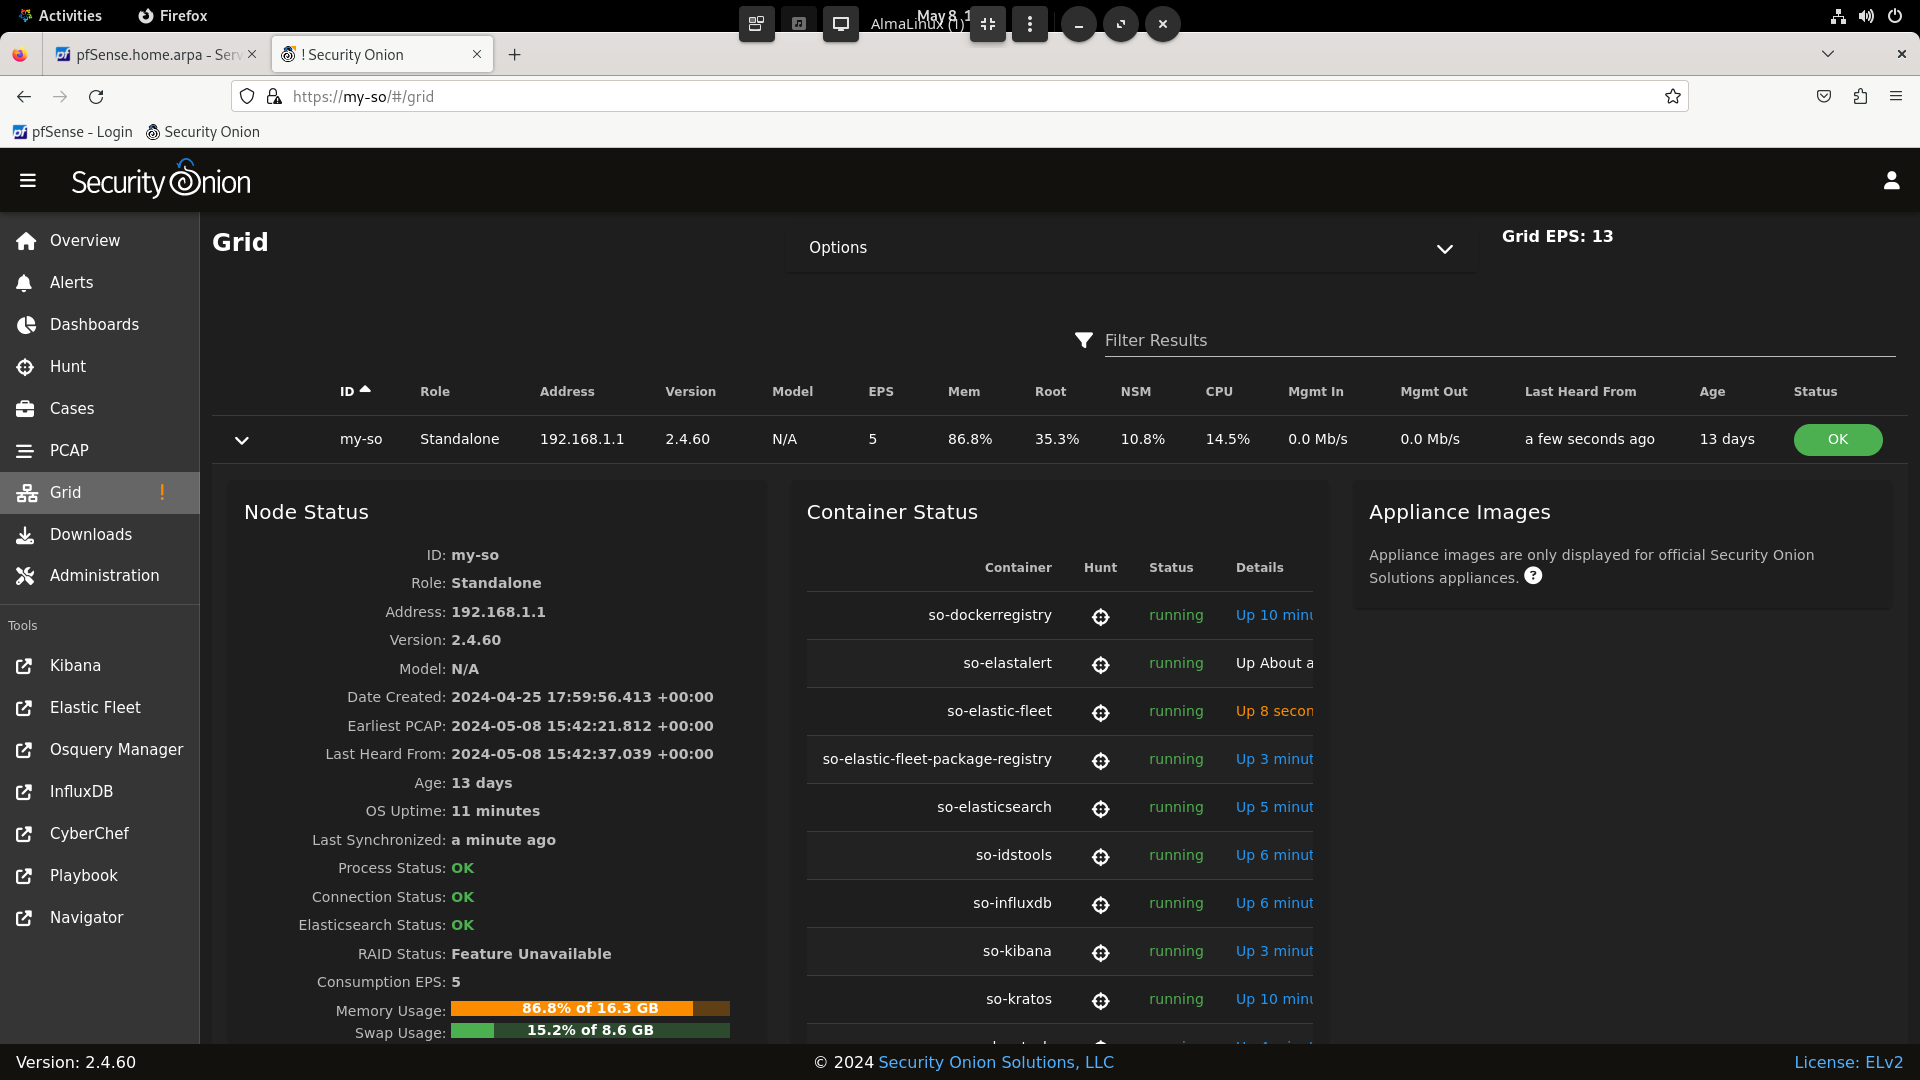
\includegraphics[width=1\textwidth]{src/assets/images/security-onion-dashboard.png}
    \caption{Dashboard of Security Onion}
\end{figure}

\subsection{Training}
Of course, since this is an academic project no real training was provided, but in a proper SoC, training and skills development are crucial for the team to be able to effectively monitor and respond to security incidents.
We might even consider hiring a third-party to provide training for the team.

This step did however manifest in the form of learning how to properly use Security Onion via the official documentation and online tutorials.

\subsection{Workflows}
This section will elaborate on the workflows that the Security Onion Essentials tutorial talks about.

\subsubsection{Alert Triage \& Case Creation}
Alerts is the first step in the process of detecting and responding to security incidents.
It contains a list of alerts that have been generated by the various detection engines in Security Onion.
In order to respond to these alerts, the analyst must first triage them to determine their severity and relevance.
After this, they can either acknowledge the alert or create a case for further investigation.

\begin{figure}[H]
    \centering
    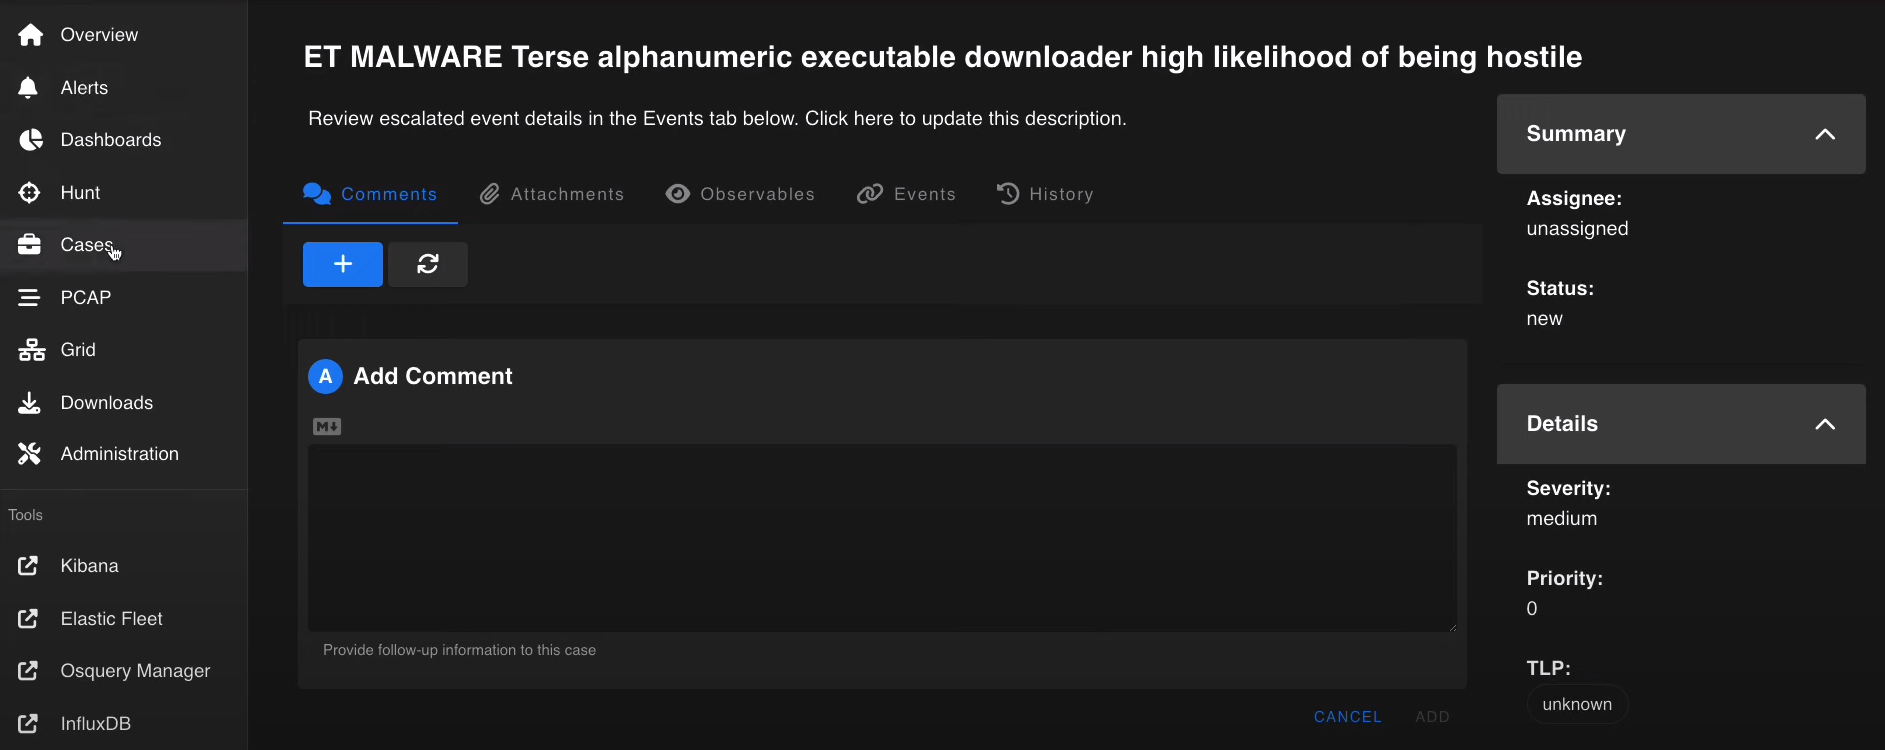
\includegraphics[width=1\textwidth]{src/assets/images/security-onion-cases.png}
    \caption{Security Onion Case Example}
\end{figure}

\subsubsection{Threat Hunting}
Hunting is where we start with a hypothesis and then search for evidence to either confirm or deny it.
This is a proactive approach to security, as opposed to the reactive approach of alert triage.

\begin{figure}[H]
    \centering
    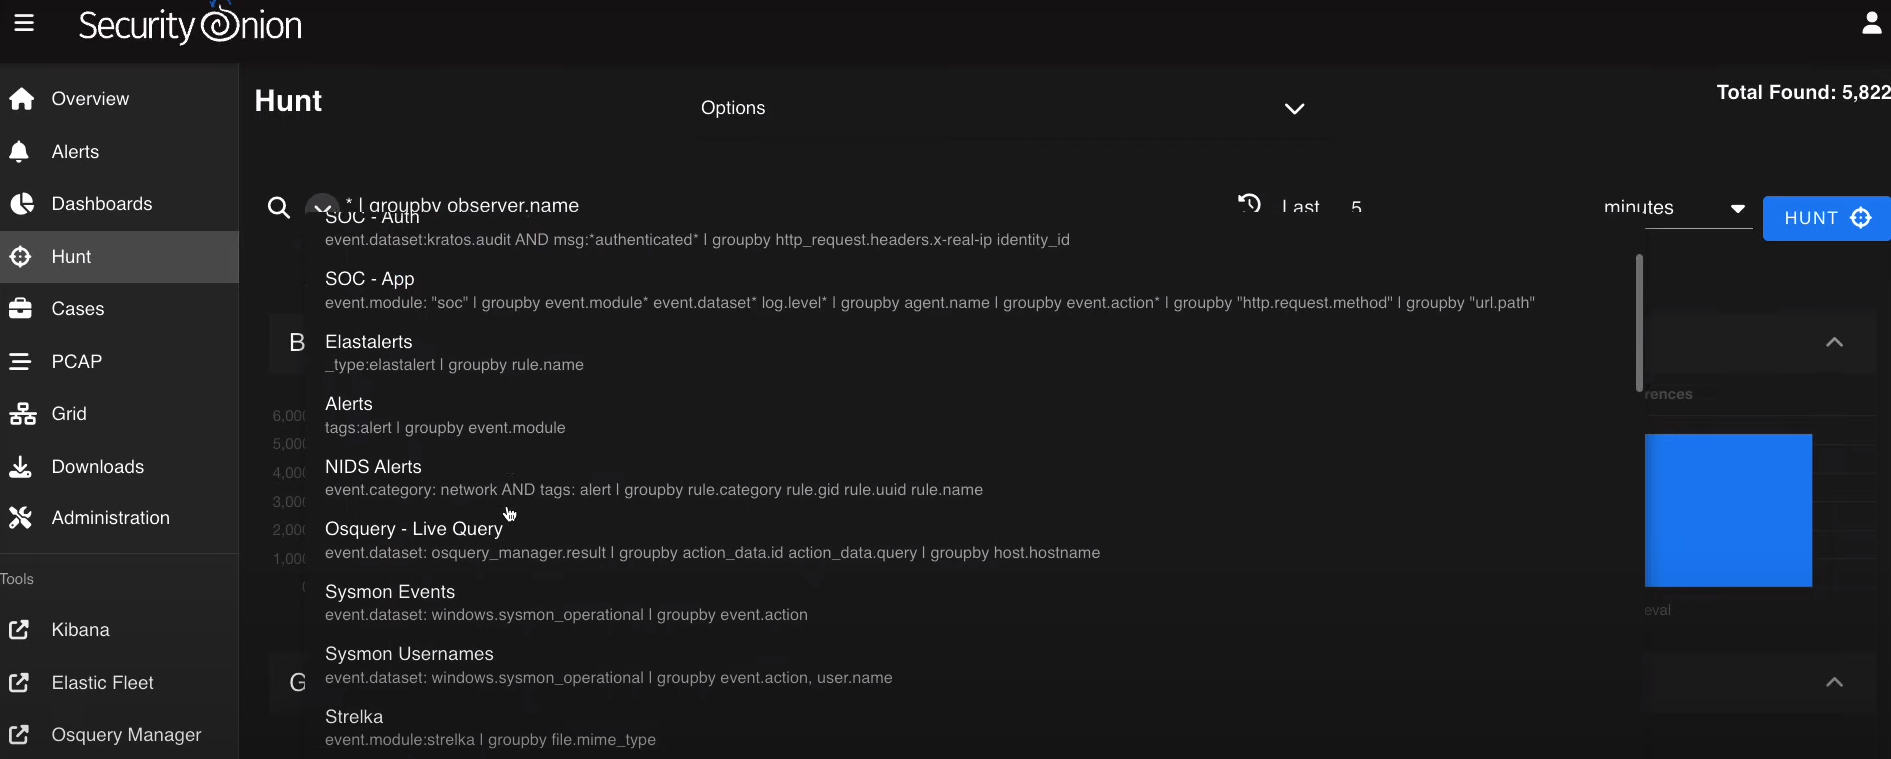
\includegraphics[width=1\textwidth]{src/assets/images/security-onion-hunt.png}
    \caption{Security Onion Hunt Example}
\end{figure}

\subsubsection{Detection Engineering}
Detection engineering is the process of developing technical means for uncovering malicious activity and misconfigurations that could lead to security incidents.
The major steps include detection gap, configuring detection pipelines, writing and testing custom rules, and finally deploying and tuning them in production.

There are many ways this can be implemented in Security Onion, but the most straightforward way is through writing Playbooks.

\begin{figure}[H]
    \centering
    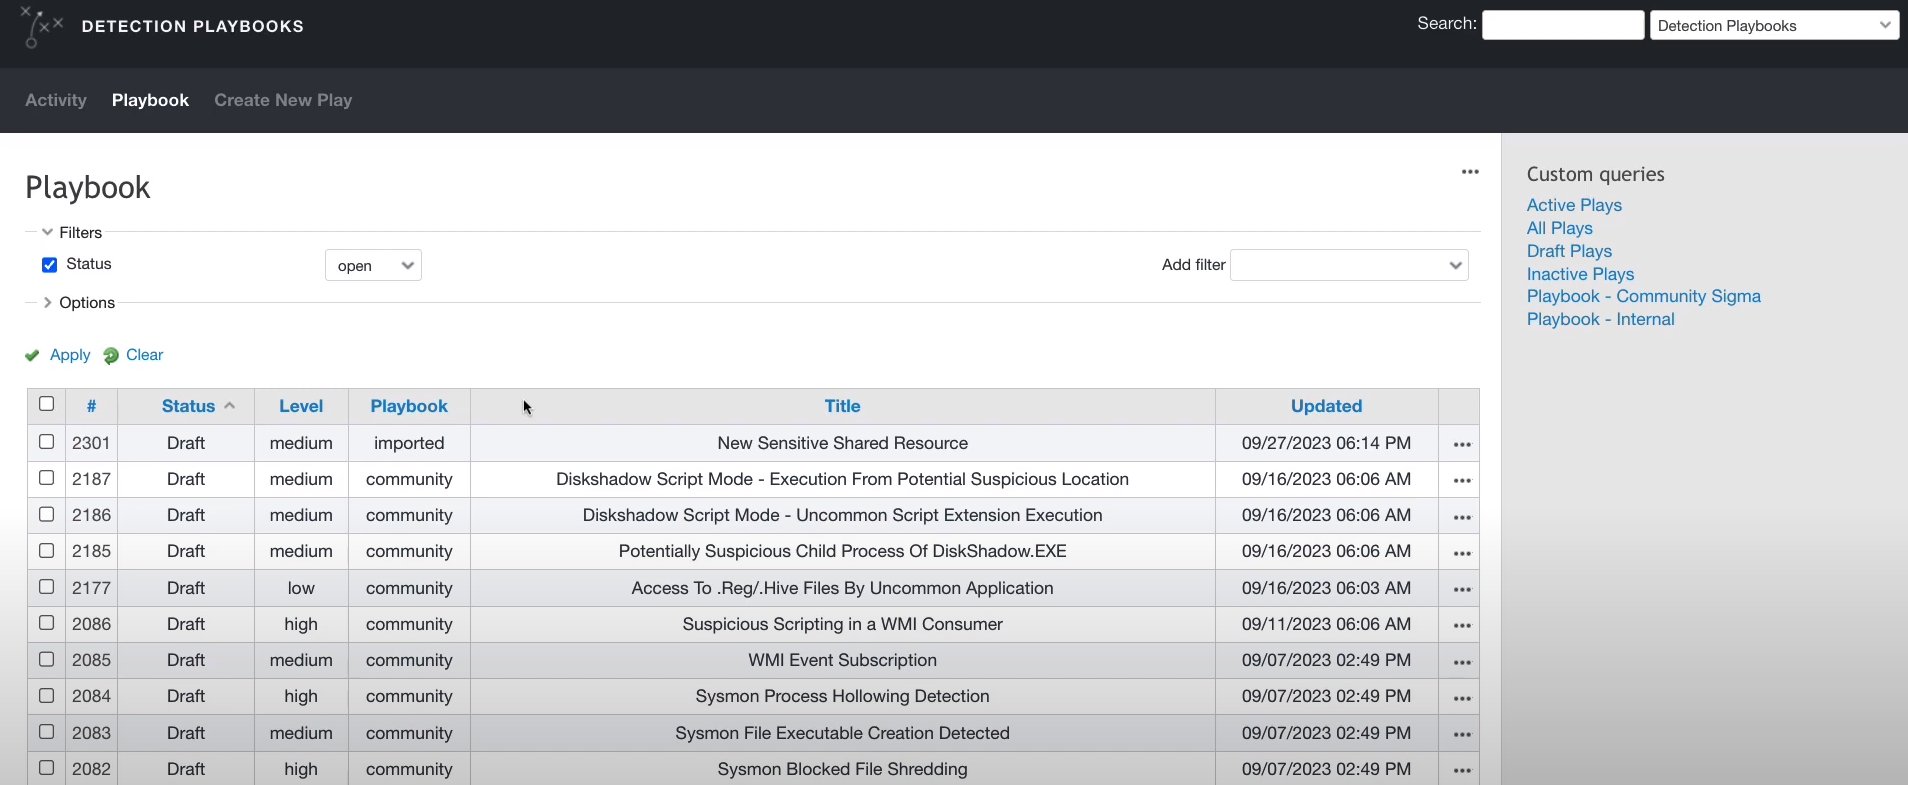
\includegraphics[width=1\textwidth]{src/assets/images/security-onion-playbooks.png}
    \caption{Security Onion Playbook Examples}
\end{figure}

Here is an example of a Sigma rule to detect the creation of new user accounts on Windows Systems using the Playbook feature in Security Onion.

\begin{figure}[H]
    \centering
    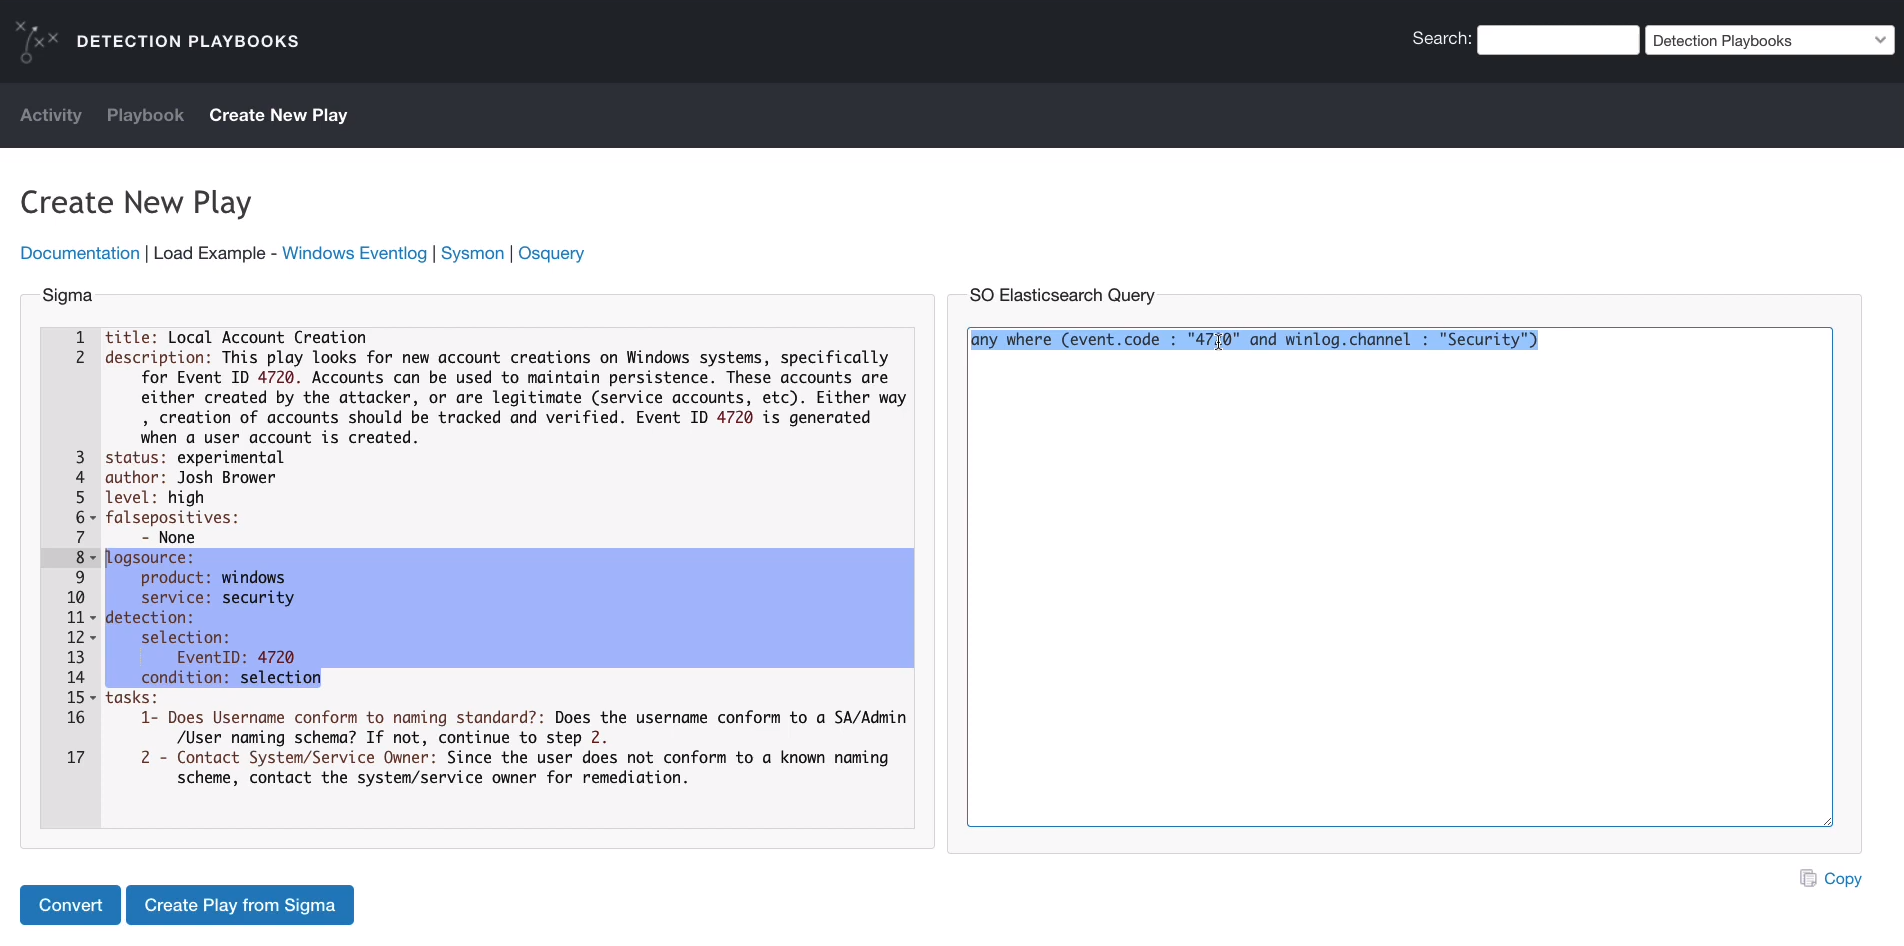
\includegraphics[width=1\textwidth]{src/assets/images/security-onion-sigma-rule.png}
    \caption{Playbook Example - User accout creation detection}
\end{figure}

% ----------------------- Technologies ----------------------- %
\section{Technologies}
This part is reserved for the presentation of all of the software used in the realization of the project and includes but is not limited to; programming languages, frameworks, technologies, etc...

\medskip
For a comparative analysis on some of our choices, see \textbf {Chapter 2: State of the art}.

\begin{itemize}
    \item \textbf{Graphical Network Simulator 3 (GNS3):} \newline The most popular network software emulator, used to emulate network devices and create any network topology \newline
          \begin{minipage}{\linewidth}
              \centering
              
\includegraphics[width=3cm]{src/assets/logos/gns3_94911_500x500.png}
              \captionof{figure}{Logo of GNS3}
          \end{minipage}
    \item \textbf{QEMU:} \newline \cite{qemu} A generic and open source machine emulator and virtualizer \newline \newline
          \begin{minipage}{\linewidth}
              \centering
              
\includegraphics[width=6cm]{src/assets/logos/qemu_logo.png}
              \captionof{figure}{Logo of QEMU}
          \end{minipage}
          \newline
    \item \textbf{Kernel-based Virtual Machine (KVM):} \newline \cite{kvm} KVM is a full virtualization solution for Linux on x86 hardware containing virtualization extensions (Intel VT or AMD-V) \newline \newline
          \begin{minipage}{\linewidth}
              \centering
              
\includegraphics[width=6cm]{src/assets/logos/kvm_banner_logo.png}
              \captionof{figure}{Logo of KVM}
          \end{minipage}
    \item \textbf{Virtual Machine Manager:} \newline \cite{kvm} A GUI used on top of QEMU/KVM \newline
          \begin{minipage}{\linewidth}
              \centering
              
\includegraphics[width=6cm]{src/assets/logos/virt-manager.png}
              \captionof{figure}{Logo of Virt Manager}
          \end{minipage}
    \item \textbf{Security Onion:} \newline A free and open source Linux distribution for threat hunting, enterprise security monitoring, and log management. \newline
          \begin{minipage}{\linewidth}
              \centering
              
\includegraphics[width=8cm]{src/assets/logos/security-onion-light.png}
              \captionof{figure}{Logo of Security Onion}
          \end{minipage}
    \item \textbf{pfSense:} \newline An open source firewall/router computer software distribution based on FreeBSD. \newline \newline
          \begin{minipage}{\linewidth}
              \centering
              
\includegraphics[width=6cm]{src/assets/logos/pfSense-640px.png}
              \captionof{figure}{Logo of pfSense}
          \end{minipage}
    \item \textbf{LaTeX:} \newline \cite{latex-project} A high-quality document preparation and typesetting system for technical grade documents. \newline \newline
          \begin{minipage}{\linewidth}
              \centering
              \includegraphics[width=4cm]{src/assets/logos/latex_200x200.png}
              \captionof{figure}{Logo of The LaTeX Project}
          \end{minipage}
\end{itemize}

% ----------------------- Difficulties encountered ----------------------- %
\section{Difficulties encountered}
\subsection{Security Onion installation}
Since the release of Security Onion 2, the installation process has changed significantly.
That heavily impacted the initial setup, especially considering that GNS3 does not support Security Onion 2 out of the box, at least at the time of writing this report.
Additionally, the new version needed 200GB of disk space, which was a challenge to allocate in the virtual machine without affecting the performance of the host machine.

The solution was to create a custom appliance with an empty qcows2 disk image of dynamically allocated storage.
What's more, a specific flag (-cpu host) was necessary for the Secuity Onion 2 QEMU virtual machine to run in graphical mode for the installation to continue.

\subsection{Networking with GNS3}
Network with GNS3 was also a major problem initially, especially when trying to reach the internet from within the emulated network.

The solution was to create a virtual bridge with libvirt (using Virt Manager) and connect the cloud node to the bridge.
Then, we had to configure the pfSense firewall to act as the gateway for the network and provide DHCP and DNS services.

\setcounter{secnumdepth}{0} % Set the section counter to 0 so next section is not counted in toc
% ----------------------- Conclusion ----------------------- %
\section{Conclusion}
In this chapter, we have discussed the implementation of the SoC using Security Onion and GNS3.
We have covered the setup of the network environment, the installation and configuration of Security Onion, and the training and skills development for the team.
We also took a look at the workflows and technologies used in the project.
Finally, we discussed the difficulties encountered during the implementation and how they were resolved.
